\documentclass[12pt,a4paper]{report}

\usepackage{amsmath}
\usepackage{amsfonts}
\usepackage{amssymb}
\usepackage{graphicx}
\usepackage{subcaption}
\usepackage{tabularx}
\usepackage{array}
\usepackage{booktabs}
\usepackage[utf8]{vietnam}
\usepackage[english]{babel}
\usepackage{enumitem}
\usepackage{float}
\usepackage{caption}
\usepackage{xcolor}
\usepackage{hyperref}
\usepackage{microtype}
\usepackage{setspace}
\usepackage{indentfirst}
\usepackage{sectsty}
\usepackage{fancyhdr}
\usepackage{tikz}
\usetikzlibrary{arrows.meta,positioning,shapes.geometric,fit}
\usepackage[left=2.5cm,right=2.2cm,top=2.4cm,bottom=2.4cm]{geometry}

\hypersetup{
    colorlinks=true,
    linkcolor=black,
    citecolor=black,
    urlcolor=blue,
    pdftitle={NLBSE'24 GitHub Issue Classification},
    pdfauthor={Seminar 2 Project Group}
}

\captionsetup{font=small,labelfont=bf}
\captionsetup[subfigure]{labelformat=empty}
\chapternumberfont{\LARGE}
\chaptertitlefont{\LARGE}
\sectionfont{\large}
\setstretch{1.12}
\setlength{\parindent}{0.6cm}
\setlength{\parskip}{0.15em}

\pagestyle{fancy}
\fancyhf{}
\lhead{\textit{Seminar 2}}
\rhead{\textit{NLBSE'24 GitHub Issue Classification}}
\cfoot{\thepage}
\renewcommand{\headrulewidth}{0.6pt}
\renewcommand{\footrulewidth}{0pt}
\setlength{\headheight}{15pt}

\definecolor{codegray}{gray}{0.93}
\newcommand{\code}[1]{\colorbox{codegray}{\texttt{#1}}}
\renewcommand{\bibname}{References}

\begin{document}

\begin{titlepage}
\thispagestyle{empty}
\begin{center}
    {\Large Hanoi University of Science and Technology\\[0.2cm]}
    {\Large School of Information and Communication Technology}

    \vspace{1.5cm}
    
\includegraphics[width=0.22\textwidth]{image/bachkhoa.png}

    \vspace{1.0cm}
    {\Large \textbf{SEMINAR 2 PROJECT REPORT}}\\[0.6cm]
    {\Huge \textbf{NLBSE'24 GitHub Issue Classification}}

    \vspace{1.4cm}
    \begin{tabular}{ll}
        \textbf{Student} & \textbf{Student ID} \\
        Pham Tuan Kiet & 20252751M \\
        Nguyen Trung Hieu & 20261059M \\
        Le Ngoc Anh & 20252275M \\
        Nguyen Hoang Nam & 20261081M \\
        Bui Tien Dung & 20261204M \\
    \end{tabular}

    \vfill
    {\Large September 25, 2026}
\end{center}
\end{titlepage}

\pagenumbering{roman}

\chapter*{Acknowledgement}
\addcontentsline{toc}{chapter}{Acknowledgement}
We would like to express our sincere appreciation to Prof. Nguyen Thanh Phuong for giving us the opportunity to work on this project. We are grateful for the helpful advice, feedback, and guidance provided throughout the project.

\chapter*{Abstract}
\addcontentsline{toc}{chapter}{Abstract}
GitHub issue triage is an important software-maintenance task in which incoming reports must be categorized before they can be prioritized, routed, and resolved. This project studies the NLBSE'24 issue classification task, where each issue is classified as a bug, feature request, or question. The dataset contains 1,500 training issues and 1,500 official test issues collected from five repositories: bitcoin/bitcoin, facebook/react, microsoft/vscode, opencv/opencv, and tensorflow/tensorflow. We compare several families of text-classification methods, including TF-IDF with Logistic Regression, LinearSVC, Complement Naive Bayes, hashed SGD, supervised fastText, RoBERTa full fine-tuning, RoBERTa with LoRA, and SetFit with MPNet and MiniLM. Experiments use repository-specific cross-validation, pooled cross-validation, leave-one-repository-out evaluation, and official test evaluation, although not every model family was evaluated under every protocol (the dense models were evaluated under cross-validation only, and RoBERTa also under pooled cross-validation). Under repository-specific cross-validation, the TF-IDF + Logistic Regression baseline obtains a mean repository-level Macro-F1 of 0.7636. SetFit MPNet reaches 0.7953, and a five-iteration SetFit configuration reaches 0.7976. RoBERTa LoRA obtains 0.7994 under pooled cross-validation, while the baseline drops to 0.5876 under leave-one-repository-out evaluation. In addition to predictive performance, the report considers computational cost and the effect of the evaluation protocol on result interpretation. Overall, pretrained dense representations achieve strong classification performance, while sparse methods remain practical alternatives when simplicity and computational efficiency are important.

\clearpage
\tableofcontents
\clearpage
\pagenumbering{arabic}

\chapter{Introduction}
Software issue trackers contain a large amount of operational knowledge about software systems. Users and developers create issues to report incorrect behavior, request new functionality, or ask for help. Before maintainers can respond effectively, these reports often need to be categorized and routed to an appropriate workflow. For large open-source projects, manually reading and labeling every incoming issue is time-consuming and can also lead to inconsistent categorization.

Automatic issue classification is therefore a natural Natural Language Processing (NLP) task. Unlike conventional short-text classification, GitHub issues may contain ordinary prose together with source code, stack traces, file paths, URLs, version numbers, command output, and repository-specific terminology. These elements can provide useful signals, but they also make the input heterogeneous and more difficult to model.

A further challenge is the difference between software repositories. Each project has its own terminology, issue templates, coding conventions, and community practices. A classifier may perform well when training and validation issues come from the same repository while transferring less effectively to a repository that was not observed during training.

This project studies the NLBSE'24 GitHub Issue Classification task \cite{nlbse2024issue}. Given the title and body of an issue, the objective is to predict one of three labels: \textit{bug}, \textit{feature}, or \textit{question}. We evaluate classical sparse models, lightweight text classifiers, pretrained Transformer models, parameter-efficient fine-tuning, and Sentence Transformer approaches within a shared experimental pipeline.

\section{Project Objectives}
The project has three practical objectives:
\begin{itemize}[leftmargin=1.5em]
    \item compare several text-classification approaches, from TF-IDF-based baselines to pretrained dense encoders;
    \item evaluate how model behavior changes across repository-specific, pooled, cross-repository, and official test settings; and
    \item consider predictive performance together with computational cost and implementation complexity.
\end{itemize}

The primary evaluation metric is Macro-F1. Because the dataset contains five repositories, performance is preserved at repository level before being summarized. Results from repository-specific cross-validation, pooled cross-validation, leave-one-repository-out evaluation, and the official test split are reported separately because these protocols answer different practical questions and use different training conditions.

\section{Report Organization}
Chapter 2 summarizes the model families used in the project. Chapter 3 describes the dataset, preprocessing choices, and evaluation protocols. Chapter 4 presents the common implementation pipeline and model-specific configurations. Chapter 5 reports the experimental results and discusses the main observations and limitations. Chapter 6 concludes the report and identifies possible improvements for future work.


\chapter{Background and Model Families}
\section{Traditional Text Classification}
Traditional text classification provides an important reference point for the GitHub issue classification task because it offers a simple and efficient way to transform textual reports into numerical features. In this family of methods, issue text is represented as a high-dimensional sparse vector, typically using Term Frequency--Inverse Document Frequency (TF-IDF). Word n-grams can capture short expressions such as ``feature request'' or ``fails to compile'', while character n-grams can preserve useful fragments from identifiers, stack traces, file paths, package names, and version strings.

The main classical baseline in this project combines TF-IDF with Logistic Regression. The lightweight-model experiments additionally evaluate LinearSVC, Complement Naive Bayes, a hashing-based SGD classifier, and supervised fastText. fastText provides an efficient neural text-classification approach based on word and subword information \cite{joulin2017bag}. These models provide useful alternatives when training time, inference cost, and memory requirements are important.

Sparse models are attractive because they can usually be trained and evaluated much more cheaply than large pretrained encoders. Their main limitation is that they rely strongly on lexical patterns and have less ability to represent contextual meaning. Two issues expressing a similar intent with different vocabulary may therefore appear distant in sparse feature space. In this report, traditional models are used both as practical classifiers and as reference systems for evaluating the additional value of pretrained representations.

\section{Transformer Architecture}
The Transformer architecture replaces recurrent sequence processing with attention-based operations, enabling substantial parallelism during training and providing a flexible mechanism for modeling relationships between tokens \cite{vaswani2017attention}. The complete architecture contains encoder and decoder stacks; for this project, the most relevant component is the encoder because RoBERTa is an encoder-only Transformer model.

\begin{figure}[H]
    \centering
    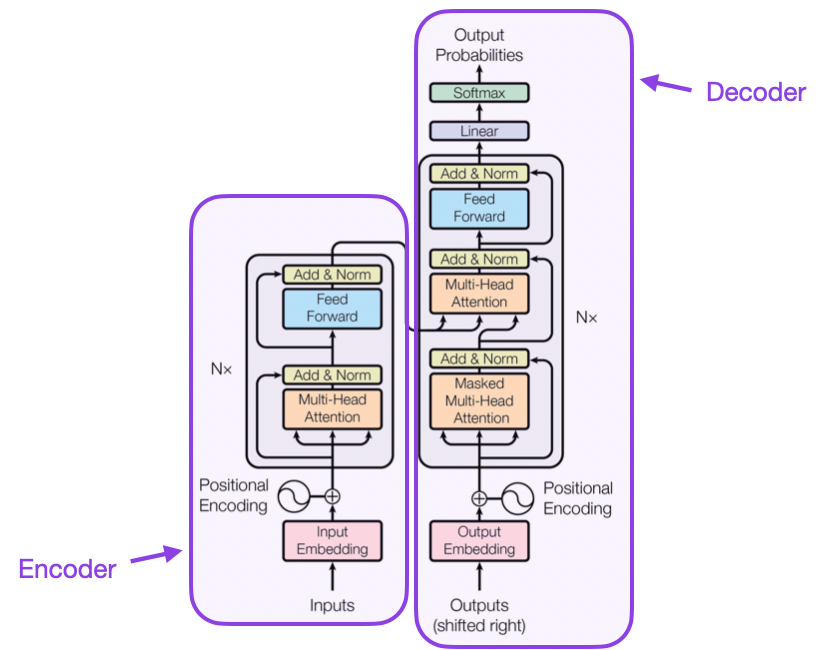
\includegraphics[width=0.52\textwidth]{image/transformer_clean.png}
    \caption{Transformer encoder--decoder architecture, adapted from Vaswani et al. \cite{vaswani2017attention}.}
    \label{fig:transformer-architecture}
\end{figure}

The main mechanisms relevant to this project are summarized below.
\begin{itemize}[leftmargin=1.5em]
    \item \textbf{Self-attention:} each token can attend to other tokens in the same sequence through query, key, and value projections. This allows the representation of a token to depend on its surrounding context.
    \item \textbf{Multi-head attention:} several attention operations are performed in parallel, allowing different heads to capture different relationships in the input.
    \item \textbf{Positional information:} because attention alone does not encode token order, positional information is added so that the model can distinguish different positions in the sequence.
    \item \textbf{Feed-forward and residual blocks:} attention layers are followed by position-wise feed-forward networks together with residual connections and normalization.
\end{itemize}

These mechanisms allow Transformer encoders to construct context-dependent token representations and make them suitable for downstream text-classification tasks.

\section{RoBERTa}
RoBERTa is a Transformer-based language model developed by revisiting and optimizing the pretraining procedure used by BERT \cite{liu2019roberta}. It retains the bidirectional Transformer encoder structure while changing several pretraining choices. In particular, RoBERTa removes the Next Sentence Prediction objective, uses dynamic masking, and is trained with more data and larger training configurations than the original BERT setup.

For downstream text classification, a pretrained RoBERTa encoder is combined with a task-specific classification head. The input is tokenized into subword units, processed by the encoder, and converted into class scores for the target labels. During full fine-tuning, both the pretrained encoder and the classification head are updated on the task data. This approach provides a direct way to adapt contextual language representations to GitHub issue classification.

\section{Low-Rank Adaptation (LoRA)}
Low-Rank Adaptation (LoRA) is a parameter-efficient fine-tuning method that adapts a pretrained model without updating all of its original parameters \cite{hu2021lora}. Instead of replacing a pretrained weight matrix $W_0$, LoRA learns a low-rank update
\begin{equation}
    \Delta W = BA,
\end{equation}
where $A$ and $B$ are smaller trainable matrices with rank $r$ much smaller than the original matrix dimensions. The forward computation can be written conceptually as
\begin{equation}
    h = W_0x + BAx.
\end{equation}

Because the pretrained weights remain frozen, only the low-rank adapters and task-specific components need to be optimized. This can reduce the number of trainable parameters and the memory required during adaptation. In this project, LoRA is evaluated as a practical alternative to full RoBERTa fine-tuning while keeping the same task and input representation.

\section{Sentence Transformers and SetFit}
Sentence Transformers are designed to produce fixed-dimensional embeddings for complete sentences or text passages. Sentence-BERT (SBERT) uses Siamese or triplet Transformer structures to produce semantically meaningful sentence representations that can be compared efficiently with similarity measures such as cosine similarity \cite{reimers2019sentencebert}.

SetFit builds on Sentence Transformers and provides a two-stage approach to text classification \cite{tunstall2022setfit}. First, a pretrained sentence encoder is adapted using contrastive learning on pairs constructed from the labeled examples. Second, the adapted encoder produces dense sentence embeddings, and a lightweight classification head is trained on those embeddings. This separation between representation learning and classification makes SetFit particularly suitable for experiments involving limited labeled data and resource-aware training.

The project evaluates two SetFit backbones: MPNet and MiniLM. MPNet provides a larger sentence-embedding model, whereas MiniLM offers a more compact alternative. Additional experiments vary the number of labeled examples and the number of contrastive-training iterations to examine data efficiency and training-cost trade-offs.


\chapter{Dataset and Evaluation Setup}
\section{Dataset Overview}
The project uses the official NLBSE'24 issue-report classification dataset \cite{nlbse2024issue}. The dataset contains two official splits, each with 1,500 issues. Five repositories are represented: bitcoin/bitcoin, facebook/react, microsoft/vscode, opencv/opencv, and tensorflow/tensorflow. For each repository, the dataset contains 100 bug issues, 100 feature issues, and 100 question issues in each official split.

\begin{table}[H]
\centering
\caption{Summary of the NLBSE'24 issue-classification dataset.}
\label{tab:dataset-summary}
\begin{tabularx}{\textwidth}{>{\bfseries}l X}
\toprule
Property & Value \\
\midrule
Training split & 1,500 issues \\
Official test split & 1,500 issues \\
Repositories & bitcoin/bitcoin; facebook/react; microsoft/vscode; opencv/opencv; tensorflow/tensorflow \\
Labels & bug; feature; question \\
Class balance & 100 examples per label and repository in each split \\
Input fields & title and body \\
\bottomrule
\end{tabularx}
\end{table}

The balanced construction in Table~\ref{tab:dataset-summary} is useful for evaluation because each target class has the same number of examples within each repository. Consequently, class-frequency imbalance is not the main source of performance differences in this dataset.

\section{Dataset Characteristics and Challenges}
Although the label distribution is balanced, the textual content is heterogeneous. Issue bodies may contain long technical descriptions, code fragments, stack traces, URLs, paths, and project-specific vocabulary. In addition, the same linguistic form can express different intents: a question may contain terms associated with a software defect, while a feature request may itself be phrased as a question.

The project therefore considers the following dataset-related challenges:
\begin{itemize}[leftmargin=1.5em]
    \item \textbf{Repository-specific language:} templates, terminology, and writing conventions differ across repositories, which can make transfer to an unseen repository more difficult.
    \item \textbf{Duplicate leakage:} identical normalized issue text should not be placed in both training and validation partitions of the same cross-validation experiment.
    \item \textbf{Technical content:} code fragments, paths, identifiers, and version strings may be informative and should not automatically be removed as noise.
    \item \textbf{Intent overlap:} the \textit{question} label can overlap linguistically with both bug reports and feature requests.
    \item \textbf{Train--test overlap checks:} exact or near-exact overlap between official splits should be inspected when interpreting final test performance.
\end{itemize}

\section{Exploratory Data Analysis}
The first EDA step is to verify the dataset structure and label distribution. Because every repository contains the same number of examples for the three labels, the class distribution is uniform by construction. Repository-level inspection remains important because issue length, issue templates, writing style, and technical vocabulary can vary substantially between projects.

In this report, EDA is used mainly to validate the split structure and identify properties that influence preprocessing and evaluation. Model-performance differences between repositories are discussed later in Chapter 5 rather than being treated as part of the dataset analysis.

The dataset audit found three shared normalized title-and-body keys across official train/test, including one with conflicting labels. Train has one exact duplicate beyond unique texts; group-aware CV keeps identical full texts together. Two test bodies are missing and converted to empty strings. Training text has median 150 words, 95th percentile 536.1 words, and maximum 21,595 words. These findings motivate duplicate-aware folds and explicit truncation limits. Official scores retain the original split for comparability; no de-overlapped sensitivity score is claimed. Overlap can favor memorization, while contradictory labels can penalize consistent classifiers.

\section{Preprocessing Pipeline}
The shared text representation combines the issue title and body after whitespace normalization. Missing fields are normalized at the data-service boundary. Technical content is retained because source-code fragments, paths, stack traces, and version identifiers can contain predictive information.

For sparse models, vectorizers are fitted only on the training portion of each fold and then applied to the corresponding validation partition. For pretrained encoders, the text is processed using the tokenizer associated with the selected model and truncated according to that model's configuration. Sampling and any representation-learning step are also performed inside the training partition to avoid using validation information during preprocessing.

\section{Evaluation Protocols}
Four evaluation protocols are used because each one represents a different practical setting. Their results are reported separately and are not treated as interchangeable.

\begin{figure}[H]
\centering
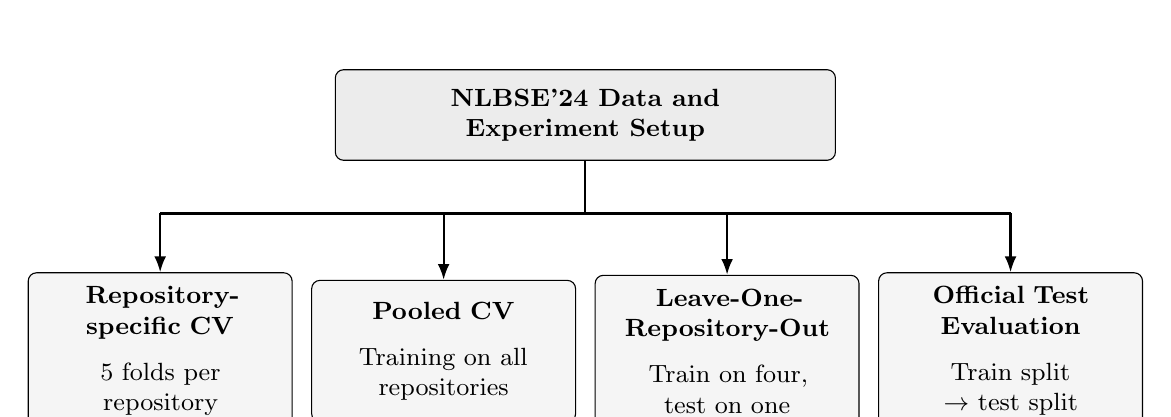
\begin{tikzpicture}[
    box/.style={
        draw,
        rounded corners=3pt,
        align=center,
        text width=3.0cm,
        minimum width=3.3cm,
        minimum height=1.8cm,
        fill=gray!8,
        inner sep=5pt,
        font=\small
    },
    mainbox/.style={
        draw,
        rounded corners=3pt,
        align=center,
        text width=6.0cm,
        minimum height=1.15cm,
        fill=gray!15,
        inner sep=5pt,
        font=\small\bfseries
    },
    arrow/.style={
        -{Latex[length=2mm]},
        thick
    }
]

% Top box
\node[mainbox] (data) at (0,3.0)
{NLBSE'24 Data and Experiment Setup};

% Four equal bottom boxes
\node[box] (cv) at (-5.4,0)
{\textbf{Repository-specific CV}\\[2mm]
5 folds per repository};

\node[box] (pooled) at (-1.8,0)
{\textbf{Pooled CV}\\[2mm]
Training on all repositories};

\node[box] (loo) at (1.8,0)
{\textbf{Leave-One-Repository-Out}\\[2mm]
Train on four, test on one};

\node[box] (official) at (5.4,0)
{\textbf{Official Test Evaluation}\\[2mm]
Train split $\rightarrow$ test split};

% Horizontal branching line
\coordinate (branch) at (0,1.75);

\draw[thick]
    (data.south) -- (branch);

\draw[thick]
    (-5.4,1.75) -- (5.4,1.75);

% Four arrows
\draw[arrow] (-5.4,1.75) -- (cv.north);
\draw[arrow] (-1.8,1.75) -- (pooled.north);
\draw[arrow] (1.8,1.75) -- (loo.north);
\draw[arrow] (5.4,1.75) -- (official.north);

\end{tikzpicture}

\caption{Overview of the evaluation protocols used in the project.}
\label{fig:evaluation-protocols}
\end{figure}

\begin{itemize}[leftmargin=1.5em]
    \item \textbf{Repository-specific Cross-Validation (CV):} for each repository, the training data is divided into five stratified folds while preserving the three-class distribution. Four folds are used for training and one for validation. Identical normalized title-and-body duplicates are grouped into the same fold to reduce leakage. This protocol measures performance when the target repository is already represented during training.

    \item \textbf{Pooled Cross-Validation:} training partitions from all five repositories are combined for each fold. The model is exposed to a broader set of repository vocabularies and writing styles, while evaluation results are still preserved at repository level before aggregation.

    \item \textbf{Leave-One-Repository-Out (LOO):} all data comes from the official training split. Each run trains on 1,200 issues from four repositories and evaluates on the remaining repository's 300 training issues. Five runs cover all held-out repositories. Official test data is not used.

    \item \textbf{Official Test Evaluation:} after configuration selection, five independent classifiers are trained, one per repository. Each uses that repository's 300 official training issues and evaluates on its 300 official test issues. This is not a pooled model trained on all 1,500 issues. Test labels must not guide further selection. Here official scores are available for P2; P1, P3 and P4 results remain training-only.
\end{itemize}

Figure~\ref{fig:evaluation-protocols} summarizes the distinction between these protocols. In particular, repository-specific CV and pooled CV should not be directly ranked against LOO or the official test setting because both the training composition and the evaluation objective differ.


\chapter{Implementation Details}
This chapter describes the implementation of the GitHub issue classification system, including the common data pipeline, model families, evaluation components, and experiment-execution process. The main goal of the implementation is to keep data handling and evaluation consistent while allowing each model family to use its own training procedure.

\section{Project Architecture}
The system is organized into components responsible for data loading, preprocessing, model training, inference, evaluation, and result storage. The dataset service reads GitHub issue records and converts them into a common representation containing the repository, issue title, issue body, and target label. The title and body are then combined into the textual input used by the selected model.

\begin{figure}[h]
\centering
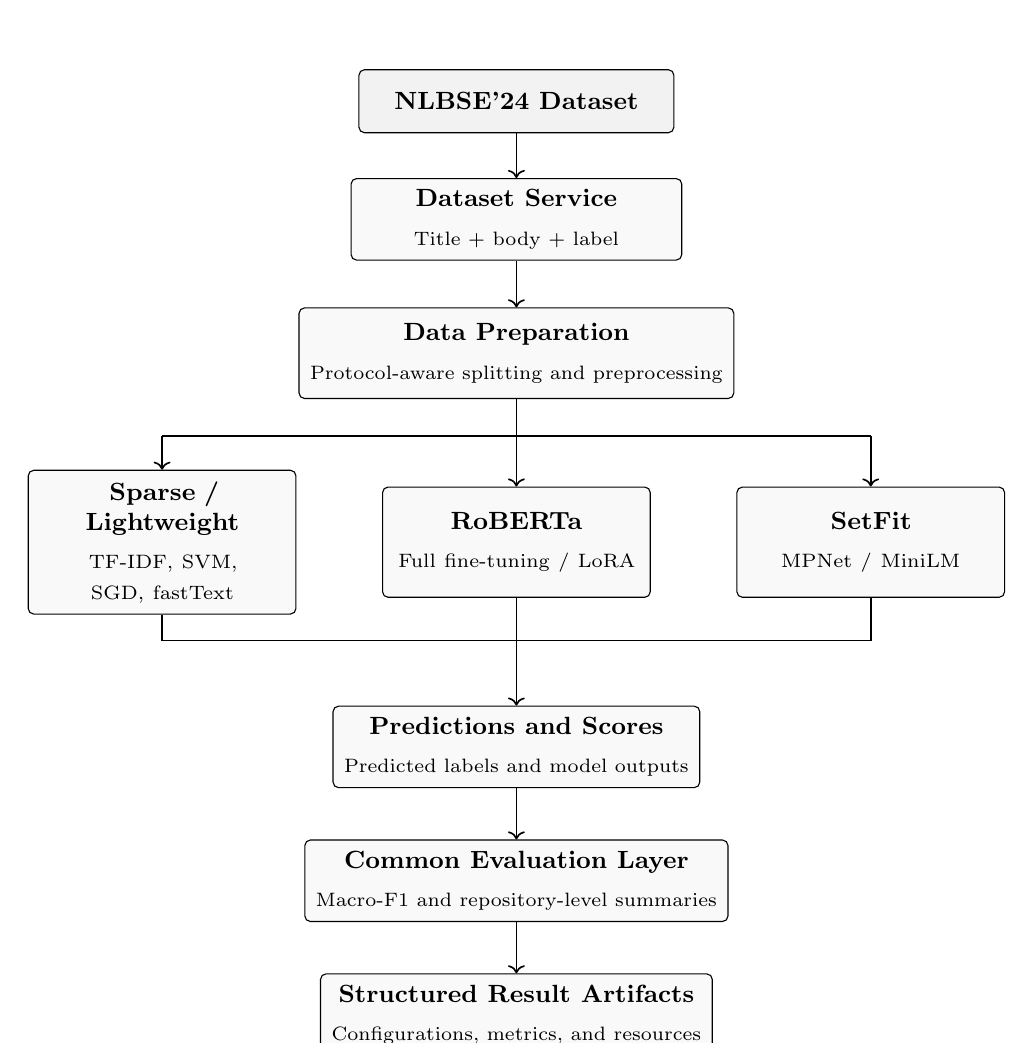
\begin{tikzpicture}[
    box/.style={
        draw,
        rounded corners=2pt,
        align=center,
        fill=gray!5,
        inner sep=4pt,
        font=\small
    },
    arrow/.style={
        ->,
        semithick
    }
]

% ==================================================
% Top pipeline
% ==================================================

\node[
    box,
    fill=gray!10,
    minimum width=4.0cm,
    minimum height=0.8cm
] (data) at (0,7.0)
{\textbf{NLBSE'24 Dataset}};


\node[
    box,
    minimum width=4.2cm,
    minimum height=1.0cm
] (service) at (0,5.5)
{
    \textbf{Dataset Service}\\[1mm]
    {\scriptsize Title + body + label}
};


\node[
    box,
    minimum width=4.2cm,
    minimum height=1.15cm
] (prep) at (0,3.8)
{
    \textbf{Data Preparation}\\[1mm]
    {\scriptsize Protocol-aware splitting and preprocessing}
};


% ==================================================
% Model boxes
% ==================================================

\node[
    box,
    text width=3.0cm,
    minimum width=3.4cm,
    minimum height=1.4cm
] (sparse) at (-4.5,1.4)
{
    \textbf{Sparse / Lightweight}\\[1mm]
    {\scriptsize TF-IDF, SVM, SGD, fastText}
};


\node[
    box,
    text width=3.0cm,
    minimum width=3.4cm,
    minimum height=1.4cm
] (roberta) at (0,1.4)
{
    \textbf{RoBERTa}\\[1mm]
    {\scriptsize Full fine-tuning / LoRA}
};


\node[
    box,
    text width=3.0cm,
    minimum width=3.4cm,
    minimum height=1.4cm
] (setfit) at (4.5,1.4)
{
    \textbf{SetFit}\\[1mm]
    {\scriptsize MPNet / MiniLM}
};


% ==================================================
% Results pipeline
% ==================================================

\node[
    box,
    minimum width=4.3cm,
    minimum height=1.0cm
] (pred) at (0,-1.2)
{
    \textbf{Predictions and Scores}\\[1mm]
    {\scriptsize Predicted labels and model outputs}
};


\node[
    box,
    minimum width=4.3cm,
    minimum height=1.0cm
] (eval) at (0,-2.9)
{
    \textbf{Common Evaluation Layer}\\[1mm]
    {\scriptsize Macro-F1 and repository-level summaries}
};


\node[
    box,
    minimum width=4.3cm,
    minimum height=1.0cm
] (artifact) at (0,-4.6)
{
    \textbf{Structured Result Artifacts}\\[1mm]
    {\scriptsize Configurations, metrics, and resources}
};


% ==================================================
% Top arrows
% ==================================================

\draw[arrow] (data.south) -- (service.north);
\draw[arrow] (service.south) -- (prep.north);


% ==================================================
% Split into three model families
% ==================================================

% Vertical stem
\draw[semithick] (prep.south) -- (0,2.75);

% Horizontal branch
\draw[semithick] (-4.5,2.75) -- (4.5,2.75);

% Arrows down to models
\draw[arrow] (-4.5,2.75) -- (sparse.north);
\draw[arrow] (0,2.75) -- (roberta.north);
\draw[arrow] (4.5,2.75) -- (setfit.north);


% ==================================================
% Merge model outputs
% ==================================================

% Vertical outputs from models
\draw[semithick] (sparse.south) -- (-4.5,0.15);
\draw[semithick] (roberta.south) -- (0,0.15);
\draw[semithick] (setfit.south) -- (4.5,0.15);

% Horizontal merge line
\draw[semithick] (-4.5,0.15) -- (4.5,0.15);

% Arrow to predictions
\draw[arrow] (0,0.15) -- (pred.north);


% ==================================================
% Final pipeline
% ==================================================

\draw[arrow] (pred.south) -- (eval.north);
\draw[arrow] (eval.south) -- (artifact.north);

\end{tikzpicture}

\caption{High-level architecture of the experimental pipeline.}
\label{fig:project-architecture}
\end{figure}

The experiment pipeline separates data preparation from model-specific training. After the dataset is loaded, the selected evaluation protocol determines how training and validation examples are divided. Components that learn from the data, such as TF-IDF vectorizers, are fitted only on the training partition of each experiment. Figure~\ref{fig:project-architecture} shows how the different model families share the same data and evaluation layers.

A common evaluation component is applied after inference. Predictions are associated with their original issue identifiers, repositories, folds, and target labels before metrics are calculated. Experimental outputs are stored as structured artifacts containing model configurations, predictions, scores, resource measurements, and environment information. This organization reduces manual copying of results and makes later comparison easier.

\section{Persistence and Team Contributions}
The \texttt{IssueRepository} abstraction is shared by in-memory, CSV and JSON adapters. \texttt{IssueDatasetService} and the runner consume this interface, so changing persistence does not require changing model/evaluation logic. This implements interchangeable memory/file storage.

\begin{table}[H]
\centering\small
\caption{Implementation ownership; each member also owns their module's analysis.}
\begin{tabularx}{\textwidth}{l l X}
\toprule
Owner & Member & Contribution \\
\midrule
P1 & Pham Tuan Kiet & Leadership; data/persistence, splits, contracts, Logistic Regression and text ablations. \\
P2 & Nguyen Trung Hieu & Sparse models, fastText, tuning and feature ablations. \\
P3 & Le Ngoc Anh & RoBERTa full/LoRA, per-repository and pooled experiments. \\
P4 & Nguyen Hoang Nam & SetFit MPNet/MiniLM, few-shot and iteration ablations. \\
P5 & Bui Tien Dung & Aggregation, paired comparisons, ensemble/resource utilities, demo and report integration. \\
\bottomrule
\end{tabularx}
\end{table}

\section{TF-IDF Logistic Regression Baseline}
The baseline classifier uses TF-IDF to transform issue text into a sparse numerical representation. The title and body are concatenated before feature extraction. Word-level unigrams and bigrams are used so that the representation can capture both individual technical terms and short phrases that may indicate issue intent. The TF-IDF vectorizer is fitted exclusively on the training portion of each fold and is then applied to the corresponding validation data.

Logistic Regression is trained on the resulting sparse feature vectors to predict the three target classes: bug, feature, and question. This model provides a computationally inexpensive reference for evaluating whether more complex contextual models produce useful gains.

A title-only configuration is also evaluated as an ablation. The model and feature extraction procedure remain unchanged while the issue body is removed from the input. The comparison measures how much useful information is contributed by the detailed issue description.

\section{Lightweight Text Classification Models}
Several lightweight classifiers are implemented as alternatives to the Logistic Regression baseline. LinearSVC is evaluated with both word-only TF-IDF features and a combination of word and character features. Character n-grams can preserve information from source-code identifiers, file paths, error messages, package names, and version strings that may be fragmented by conventional tokenization.

Complement Naive Bayes and a hashing-based Stochastic Gradient Descent classifier provide additional sparse-learning alternatives. The hashing-based model maps textual features into a fixed-dimensional space without maintaining an explicit vocabulary. A supervised fastText model is also included as a lightweight neural approach that can use subword information.

\section{RoBERTa Full Fine-Tuning}
RoBERTa-base is used as the main pretrained Transformer classifier. Each issue is formed by concatenating its title and body before tokenization. The tokenizer converts the text into subword token identifiers and an attention mask. Input sequences are truncated to a maximum length of 160 tokens to maintain a consistent computational budget across the reported RoBERTa experiments.

For full fine-tuning, the pretrained encoder is combined with a three-class classification head. Gradients are propagated through both the classification head and the pretrained Transformer layers. RoBERTa is evaluated under repository-specific and pooled cross-validation so that repository-specific training and multi-repository training can be examined separately.

\section{RoBERTa with LoRA}
The parameter-efficient RoBERTa configuration uses LoRA adapters in selected attention projections. Most pretrained RoBERTa weights remain frozen, while the low-rank adapter parameters and task-specific classification components are optimized. The tokenizer, maximum sequence length, and three-class prediction objective are kept aligned with the full fine-tuning configuration to make the adaptation strategies easier to compare.

The LoRA configuration is evaluated in the same repository-aware framework as full RoBERTa. Repository-level results are preserved before aggregate scores are calculated.

\section{SetFit Classification}
SetFit is implemented using Sentence Transformer encoders. In the first stage, the sentence encoder is adapted through contrastive training. In the second stage, the adapted encoder generates dense embeddings and a lightweight classification head is fitted on these representations.

Two encoder backbones are considered: MPNet and MiniLM. Additional experiments vary the number of labeled training examples with $k=8$, $k=16$, and $k=32$, and vary the number of contrastive-training iterations. These configurations are used to study the relationship between data availability, additional training effort, and predictive performance.

\section{Configuration Summary}
Few-shot $k$ denotes examples \emph{per class}: 24, 48 or 96 examples per repository/fold for $k=8,16,32$. ``Full data'' uses only each CV fold's training partition (approximately 240 issues), not all 300 issues including validation.

Table~\ref{tab:configuration-summary} collects the model settings that are explicitly discussed in this report. More detailed run-specific information is stored in the experiment artifacts generated by the implementation.

\begin{table}[H]
\centering
\caption{Summary of the main reported model configurations.}
\label{tab:configuration-summary}
\begin{tabularx}{\textwidth}{>{\bfseries}l X}
\toprule
Model family & Reported configuration \\
\midrule
TF-IDF + Logistic Regression & Word unigrams and bigrams; title + body; title-only ablation \\
LinearSVC & Word-only and word + character feature variants \\
Hashed SGD & Hashing-based sparse text representation \\
fastText & Supervised word/subword text classifier \\
RoBERTa & RoBERTa-base; maximum sequence length of 160 tokens; full fine-tuning \\
RoBERTa + LoRA & Same input setup as full RoBERTa; parameter-efficient low-rank adapters \\
SetFit & MPNet and MiniLM backbones; $k \in \{8,16,32\}$ experiments; multiple contrastive-iteration settings \\
\bottomrule
\end{tabularx}
\end{table}

P1/P3/P4 runs reported here use seed 42. Logistic Regression uses word 1--2 grams, minimum document frequency 2, at most 50,000 features, $C=4$, balanced weights and LBFGS (maximum 2,000 iterations). RoBERTa uses 20 epochs, train/evaluation batches 16/32 and maximum length 160. Full fine-tuning uses learning rate $2\times10^{-5}$ and weight decay 0.1; LoRA uses $3\times10^{-4}$ and weight decay 0, rank 48, alpha 96, dropout 0.1, targeting query/key/value and attention-output dense projections. These are different recipes, so differences cannot be attributed solely to the adapter mechanism. SetFit uses maximum length 128, one epoch, encoder/head batches 16/2, and 20 iterations unless ablated. Exact configurations are versioned under \texttt{configs/}.

\section{Evaluation, Ensemble, and Resource Utilities}
All trained models are evaluated through a common component. Macro-F1 is the primary performance metric, while repository-level results are retained before aggregate summaries are computed. This avoids hiding large differences between repositories behind a single overall value.

The implementation also supports paired bootstrap analysis when two models provide predictions for the same examples. Resampling matched predictions can be used to estimate uncertainty in the observed difference between models. In addition, ensemble utilities support hard voting on predicted labels and soft voting when compatible probability outputs are available. Decision margins from models such as LinearSVC are not treated as probabilities without calibration.

Training time, inference time, and memory consumption are recorded when available. Resource measurements are interpreted cautiously because CPU/GPU hardware and the number of model-fitting operations differ across protocols. For this reason, values collected under different environments are treated as practical measurements rather than as a fully controlled benchmark.

\section{Experiment Execution}
Each experiment follows the same general sequence. The required split is created according to the selected evaluation protocol. Model-specific preprocessing is then fitted using only the training partition. The classifier is trained, predictions are generated for the validation or test partition, and the outputs are passed to the shared evaluation component. Metrics, predictions, resource measurements, and configuration information are stored together.

Repeating this process across repositories, folds, model configurations, and protocols produces the collection of artifacts used in the final analysis. The standardized procedure reduces the risk that observed differences arise from inconsistent data handling and makes the experimental workflow easier to verify and reproduce.


\chapter{Experimental Results}
This chapter presents the experimental results obtained from the different model families and evaluation protocols. The analysis focuses primarily on Macro-F1, while computational cost and repository-level differences are considered where the available measurements support such comparisons. Results from repository-specific Cross-Validation, Pooled Cross-Validation, Leave-One-Repository-Out evaluation, and Official Test Evaluation are kept separate because each protocol represents a different training and evaluation condition.

\section{Evaluation Metrics}
The primary evaluation metric is Macro-F1. For each target class $c$, Precision and Recall are defined as
\begin{equation}
    \text{Precision}_c = \frac{TP_c}{TP_c + FP_c},
\end{equation}
and
\begin{equation}
    \text{Recall}_c = \frac{TP_c}{TP_c + FN_c},
\end{equation}
where $TP_c$, $FP_c$, and $FN_c$ denote true positives, false positives, and false negatives for class $c$.

The class-level F1-score is the harmonic mean of Precision and Recall:
\begin{equation}
    F1_c = 2 \times \frac{\text{Precision}_c \times \text{Recall}_c}
    {\text{Precision}_c + \text{Recall}_c}.
\end{equation}

For the three target classes, the overall Macro-F1 is
\begin{equation}
    \text{Macro-F1} =
    \frac{F1_{\text{bug}} + F1_{\text{feature}} + F1_{\text{question}}}{3}.
\end{equation}

Macro-F1 gives equal weight to the three classes. This is useful even though the dataset is balanced because it prevents strong performance on one category from hiding weak performance on another. Unless stated otherwise, the scores reported below refer to Macro-F1.

\section{Baseline Results}
For reported CV scores, let $F_{r,k}$ be the three-class macro-F1 of repository $r$ and fold $k$. The ranking score is $\frac{1}{5}\sum_{r=1}^{5}\frac{1}{K}\sum_{k=1}^{K}F_{r,k}$, with $K=5$ for CV and pooled CV, and $K=1$ for LOO or official evaluation. It is not the F1 of predictions pooled across all repositories. Absent-class denominators use zero-division handling consistent with the shared evaluator.

The TF-IDF + Logistic Regression classifier provides the main reference point for the remaining experiments. When both title and body are used, the model obtains a repository-specific CV Macro-F1 of 0.7636. The title-only configuration obtains 0.5953, an absolute decrease of 0.1683. This result shows that the issue body provides substantial information beyond the short title.

\begin{table}[H]
\centering
\caption{Performance of the TF-IDF + Logistic Regression baseline.}
\label{tab:baseline-results}
\begin{tabular}{lcc}
\toprule
\textbf{Input} & \textbf{CV Macro-F1} & \textbf{LOO Macro-F1} \\
\midrule
Title + Body & 0.7636 & 0.5876 \\
Title Only & 0.5953 & 0.5075 \\
\bottomrule
\end{tabular}
\end{table}

Table~\ref{tab:baseline-results} also shows a large reduction when the evaluation setting changes from repository-specific CV to LOO. Under CV, training data contains examples from the same repository as the validation data. Under LOO, the target repository is completely absent from training. The difference should not be interpreted as a purely causal estimate of domain shift because the amount and composition of training data also change. Nevertheless, it indicates that transfer to an unseen repository is considerably more difficult for this baseline.

\subsection*{Updated P1 uncertainty and error analysis}
The title-only LOO run uses the frozen configuration and identical held-out repositories. Its score is 0.5075, versus 0.5876 for title plus body. A paired bootstrap with 10,000 resamples (seed 42) samples issue rows with replacement within each repository, shares draws across models, and averages repository macro-F1 equally. The observed title-plus-body advantage is $+0.0801$, with percentile 95\% CI $[0.0484,0.1120]$. Individual intervals are $[0.5621,0.6108]$ for title plus body and $[0.4814,0.5312]$ for title only.

These intervals condition on fixed trained models and five observed repositories. They exclude training variability and new-repository uncertainty. Issue rows are assumed exchangeable; duplicates or dependent issues may make intervals optimistic.

\begin{table}[H]
\centering
\caption{LOO class F1 averaged equally over repositories.}
\begin{tabular}{lrrr}
\toprule
Class & Title + body & Title only & Difference \\
\midrule
bug & 0.5463 & 0.4402 & +0.1061 \\
feature & 0.6693 & 0.5996 & +0.0697 \\
question & 0.5471 & 0.4826 & +0.0645 \\
\bottomrule
\end{tabular}
\end{table}
The largest descriptive gain is on bugs. Across 1,500 held-out predictions, true bugs predicted as questions decrease from 207 to 182, and true features predicted as bugs decrease from 74 to 29. Pooled counts are for error inspection, not computing repository-balanced F1. Full matrices and per-repository metrics are in \texttt{reports/p1\_loo\_analysis.json}.

\section{Lightweight Model Results}
The P2 scores below are transcribed from the versioned P2 findings. Their complete raw-artifact handoff is still pending, so this report revision does not claim an independent recomputation of all P2 results.
Several lightweight classifiers are evaluated as alternatives to Logistic Regression. Among the LinearSVC configurations, the word-only model obtains a CV Macro-F1 of 0.7541, while the word-and-character configuration obtains 0.7533. The difference under repository-specific CV is small, but the word-and-character variant obtains higher scores under LOO and Official Test Evaluation.

\begin{table}[H]
\centering
\caption{Performance of lightweight text-classification models.}
\label{tab:lightweight-results}
\begin{tabular}{lccc}
\toprule
\textbf{Model} & \textbf{CV} & \textbf{LOO} & \textbf{Official} \\
\midrule
Word LinearSVC & 0.7541 & 0.5898 & 0.7498 \\
Word + Character LinearSVC & 0.7533 & 0.6003 & 0.7591 \\
Hashed SGD & 0.7030 & 0.6152 & 0.7322 \\
Supervised fastText & 0.7089 & 0.5384 & 0.6896 \\
Complement Naive Bayes & 0.7054 & 0.4904 & 0.7108 \\
\bottomrule
\end{tabular}
\end{table}

As shown in Table~\ref{tab:lightweight-results}, Hashed SGD obtains a CV Macro-F1 of 0.7030 but reaches 0.6152 under LOO, the highest LOO value among the lightweight configurations listed here. The relative ordering of lightweight models therefore changes across evaluation settings, reinforcing the need to keep protocol labels attached to every score.

Character features also introduce additional computational cost. The reported word-and-character LinearSVC configuration requires approximately 8.5 times the fitting time and 11.5 times the inference time of the word-only configuration. The small predictive difference should therefore be interpreted together with this additional cost.

\section{RoBERTa Results}
Full RoBERTa fine-tuning and LoRA produce similar aggregate performance under repository-specific CV, but their behavior differs across individual repositories. Full fine-tuning obtains a mean repository-level Macro-F1 of 0.7853, compared with 0.7800 for LoRA.

\begin{table}[H]
\centering
\caption{Repository-level Macro-F1 of RoBERTa full fine-tuning and LoRA under repository-specific CV.}
\label{tab:roberta-repo-results}
\begin{tabular}{lccc}
\toprule
\textbf{Repository} & \textbf{Full} & \textbf{LoRA} & \textbf{Difference} \\
\midrule
bitcoin/bitcoin & 0.7351 & 0.7345 & -0.0006 \\
facebook/react & 0.8076 & 0.8316 & +0.0240 \\
microsoft/vscode & 0.7407 & 0.7562 & +0.0155 \\
opencv/opencv & 0.7632 & 0.7533 & -0.0099 \\
tensorflow/tensorflow & 0.8797 & 0.8247 & -0.0550 \\
\midrule
Cross-Repository Mean & 0.7853 & 0.7800 & -0.0052 \\
\bottomrule
\end{tabular}
\end{table}

Table~\ref{tab:roberta-repo-results} shows that the aggregate mean hides meaningful repository-level variation. LoRA produces higher scores on React and VS Code, whereas full fine-tuning is higher on Bitcoin, OpenCV, and especially TensorFlow. The effect of the adaptation strategy is therefore not consistent across repositories.

Under Pooled Cross-Validation, full fine-tuning obtains a Macro-F1 of 0.7924 and LoRA obtains 0.7994. This relationship differs from repository-specific CV, where full fine-tuning has the slightly higher aggregate value. Because pooled and repository-specific CV use different training compositions, the two settings are reported separately rather than combined into a single ranking.

\section{SetFit Results}
SetFit achieves strong repository-specific CV performance across several configurations. The full-data MPNet configuration with 20 contrastive iterations obtains a Macro-F1 of 0.7953, while the corresponding MiniLM configuration reaches 0.7881. MiniLM requires substantially less fitting time in the reported environment: 55.1 seconds compared with 145.4 seconds for MPNet.

\begin{table}[H]
\centering
\caption{Performance and resource measurements of SetFit configurations.}
\label{tab:setfit-results}
\resizebox{\textwidth}{!}{
\begin{tabular}{lcccc}
\toprule
\textbf{Configuration} & \textbf{Macro-F1} & \textbf{Fit Time (s)} & \textbf{Inference (s)} & \textbf{Memory proxy (MiB)} \\
\midrule
MPNet, Full Data, 20 Iterations & 0.7953 & 145.4 & 0.23 & 2594 \\
MiniLM, Full Data, 20 Iterations & 0.7881 & 55.1 & 0.07 & 2655 \\
MPNet, $k=8$ & 0.6785 & 22.9 & 0.19 & 2199 \\
MPNet, $k=16$ & 0.7375 & 35.0 & 0.20 & 2318 \\
MPNet, $k=32$ & 0.7833 & 60.9 & 0.20 & 2476 \\
MPNet, 5 Iterations & 0.7976 & 44.2 & 0.23 & 2521 \\
MPNet, 80 Iterations & 0.7970 & 533.6 & 0.21 & 2505 \\
\bottomrule
\end{tabular}
}
\end{table}

The sampling experiments in Table~\ref{tab:setfit-results} show a clear improvement as the number of labeled training examples increases. MPNet obtains 0.6785 with $k=8$, 0.7375 with $k=16$, and 0.7833 with $k=32$. The result indicates that classification quality remains sensitive to labeled-data availability even when pretrained sentence representations are used.

The contrastive-iteration experiment shows a different pattern. Five iterations obtain a Macro-F1 of 0.7976 with a fitting time of 44.2 seconds, whereas 80 iterations obtain 0.7970 while requiring 533.6 seconds. In this experiment, the much longer run does not provide a corresponding performance improvement, demonstrating diminishing returns from additional contrastive-training iterations.

In the SetFit table, times are means over 25 repository/fold evaluations, not the total experiment time. The memory column preserves the original report's proxy: the mean of $\max(\texttt{python\_peak\_mb},\texttt{rss\_after\_mb})$ during fit. For MPNet this is 2594.15 MiB. RSS is sampled after fit rather than continuously, while the Python peak measures traced Python allocations only. This proxy is \emph{not peak process RAM or GPU VRAM}. SetFit runs used the reported RTX PRO 6000 Blackwell environment; no controlled cross-family resource ranking is claimed.

\section{Overall Model Comparison}
Table~\ref{tab:cv-main-comparison} compares the principal models under the same repository-specific CV protocol. Within this setting, pretrained dense models obtain higher observed Macro-F1 values than the TF-IDF + Logistic Regression baseline, although the differences among the strongest dense configurations are relatively small.

\begin{table}[H]
\centering
\caption{Main model comparison under repository-specific cross-validation.}
\label{tab:cv-main-comparison}
\begin{tabular}{lc}
\toprule
\textbf{Model} & \textbf{Macro-F1} \\
\midrule
TF-IDF + Logistic Regression & 0.7636 \\
RoBERTa Full Fine-Tuning & 0.7853 \\
RoBERTa LoRA & 0.7800 \\
SetFit MPNet & 0.7953 \\
SetFit MPNet, 5 Iterations & 0.7976 \\
SetFit MiniLM & 0.7881 \\
\bottomrule
\end{tabular}
\end{table}

Pooled CV is shown separately in Table~\ref{tab:pooled-roberta-comparison}. This avoids visually mixing scores from different training conditions.

\begin{table}[H]
\centering
\caption{RoBERTa comparison under pooled cross-validation.}
\label{tab:pooled-roberta-comparison}
\begin{tabular}{lc}
\toprule
\textbf{Model} & \textbf{Macro-F1} \\
\midrule
RoBERTa Full Fine-Tuning & 0.7924 \\
RoBERTa LoRA & 0.7994 \\
\bottomrule
\end{tabular}
\end{table}

The pooled LoRA value of 0.7994 should not be interpreted as a direct improvement over the repository-specific CV values in Table~\ref{tab:cv-main-comparison}. Pooled training exposes the model to examples from all repositories simultaneously and therefore represents a different experimental condition.

\section{Ensemble and Resource Considerations}
We executed P5's comparison and ensemble utilities from revision \texttt{09fe724} on the versioned CV artifacts (seed 42), aligning 25 repository/fold evaluations by protocol, seed, fold, test fingerprint and ordered labels. No models were retrained. An illustrative equal-weight hard vote combines Logistic Regression and SetFit MPNet; ties use the implementation's fixed class order (bug, feature, question). No ensemble weights were tuned.

\begin{table}[H]
\centering
\caption{Post-hoc CV integration check, not an official-test result.}
\begin{tabular}{lr}
\toprule
Model & Repository-balanced macro-F1 \\
\midrule
Logistic Regression & 0.7636 \\
SetFit MPNet & 0.7953 \\
Equal-weight hard vote (LR + MPNet) & 0.7885 \\
\bottomrule
\end{tabular}
\end{table}
The ensemble improves on LR by 0.0249 but trails MPNet by 0.0068; this combination does not outperform its strongest component. Because two-model votes frequently tie, the fixed tie rule matters. This descriptive check must not be treated as an independently validated ensemble-selection procedure.

A paired bootstrap comparison of LR and MPNet uses 10,000 resamples with RNG seed 42. Rows are resampled within each aligned fold, sharing indices across models, then scores are averaged within repositories and equally across repositories. MPNet minus LR is $+0.0317$, with percentile 95\% CI $[0.0085,0.0557]$. Individual CIs are $[0.7375,0.7805]$ for LR and $[0.7705,0.8114]$ for MPNet. These intervals condition on fixed predictions and do not account for overlapping training folds, training randomness, configuration-selection optimism, or new-repository uncertainty. They are not a posterior probability that one model is universally better.

JSON outputs are supplied as \path{reports/p5_cv_comparison.json} and \path{reports/p5_cv_ensemble.json}, with exact reproduction commands in \path{reports/latex/README.md}. Soft voting remains available only for compatible probability outputs; LinearSVC margins must not be averaged as probabilities.

No global Pareto frontier is presented: legacy artifacts lack a verified common hardware identity. P5's safe default excludes unknown-hardware groups and separates protocols. Hardware must be verified or measurements recollected before presenting a controlled cross-family frontier.

Resource measurements are also interpreted within their experimental context. Training time, inference time, and memory usage can be strongly affected by the underlying CPU or GPU and by the number of fitting operations required by the protocol. Consequently, the reported resource values are useful for within-environment observations, such as the SetFit iteration comparison, but they should not be treated as a controlled benchmark across all model families.

\section{Discussion}
\subsection{Main Observations}
The experiments show a clear difference between classification within repositories already represented during training and transfer to an unseen repository. The Logistic Regression baseline decreases from 0.7636 under repository-specific CV to 0.5876 under LOO, and several lightweight classifiers show similar protocol-dependent changes. Repository-specific vocabulary, issue templates, and writing conventions therefore appear to be important factors in model behavior.

Pretrained dense representations provide strong results under repository-specific CV. RoBERTa and SetFit configurations improve on the sparse Logistic Regression baseline in the reported experiments, but the gains are moderate relative to the additional implementation and computational complexity. The SetFit iteration experiments further show that more training does not automatically lead to better predictive performance.

A practical conclusion from these results is that model choice should depend on the deployment setting. Sparse models remain attractive when simplicity, fast training, and low computational requirements are priorities. Dense pretrained models provide higher observed CV performance in this project, while parameter-efficient and sentence-embedding approaches offer alternatives to conventional full fine-tuning.

\subsection{Limitations}
Several limitations should be considered when interpreting the results. First, not every model family was evaluated with the same number of random seeds, so very small score differences should not be overinterpreted. Second, configuration selection using cross-validation can make the reported CV values optimistic when the same folds are also used for model selection. Third, computational measurements were collected under different hardware environments for some model families, which prevents a fully controlled comparison of training and inference cost. Finally, CV, pooled CV, LOO, and official test evaluation address different questions and should remain separated when conclusions are drawn from their scores.


\chapter{Conclusion}
This project investigated automatic classification of GitHub issues into bug, feature, and question categories using the NLBSE'24 dataset. The implementation compared classical sparse classifiers with pretrained Transformer and Sentence Transformer approaches within a shared data and evaluation pipeline.

The experiments show that the issue body contributes substantial information beyond the title alone. The TF-IDF + Logistic Regression baseline reaches 0.7636 Macro-F1 under repository-specific CV but decreases to 0.5876 under LOO, illustrating the difficulty of transfer to a repository that is absent from training. Under repository-specific CV, SetFit MPNet reaches 0.7953 and the five-iteration SetFit configuration reaches 0.7976. RoBERTa LoRA reaches 0.7994 under pooled CV; this result is reported separately because the pooled protocol uses a different training composition.

The title-only LOO extension reaches 0.5075. Its paired difference from title plus body supports a positive body-text contribution under the fixed-prediction bootstrap, with the largest descriptive gain on bugs. P5's illustrative LR--MPNet hard vote reaches 0.7885, below MPNet alone; combining models does not automatically improve performance. These are training-only, post-hoc analyses rather than official-test validation.

The project also highlights the importance of interpreting predictive performance together with evaluation protocol and computational cost. Sparse classifiers remain simple and inexpensive reference systems, while pretrained dense models provide stronger observed CV performance in the reported experiments. The SetFit iteration results further show that substantially longer training does not necessarily produce a better score.

The shared experiment pipeline provides a useful foundation for future extensions because it keeps data identity, model configuration, predictions, metrics, and available resource information together. Possible improvements include evaluating more pretrained models under LOO, repeating stochastic experiments with a consistent set of random seeds, collecting resource measurements on a single controlled hardware environment, and reporting additional per-class or error-analysis results. These extensions would strengthen the comparison while preserving the practical scope of the project report.


\clearpage
\renewcommand{\bibname}{References}
\bibliographystyle{plain}
\bibliography{references}

\end{document}
